\documentclass[10pt,twocolumn,letterpaper]{article}

\usepackage{cvpr}
\usepackage{times}
\usepackage{epsfig}
\usepackage{graphicx}
\usepackage{amsmath}
\usepackage{amssymb}

% Include other packages here, before hyperref.

% If you comment hyperref and then uncomment it, you should delete
% egpaper.aux before re-running latex.  (Or just hit 'q' on the first latex
% run, let it finish, and you should be clear).
\usepackage[pagebackref=true,breaklinks=true,letterpaper=true,colorlinks,bookmarks=false]{hyperref}

\cvprfinalcopy % *** Uncomment this line for the final submission

\def\cvprPaperID{****} % *** Enter the CVPR Paper ID here
\def\httilde{\mbox{\tt\raisebox{-.5ex}{\symbol{126}}}}

% Pages are numbered in submission mode, and unnumbered in camera-ready
\ifcvprfinal\pagestyle{plain}\fi
\begin{document}

%%%%%%%%% TITLE
\title{
Lightweight Sentiment Analysis: Comparing Small LLMs, Large Models, and Traditional ML Approaches

Small NLP: CS 7643
}

\author{
Jaden Zwicker, 
Houshmand Abbaszadeh,
Brieuc Popper
\\
Georgia Institute of Technology\\
Atlanta, GA 30332\\
{\tt\small 
jzwicker3@gatech.edu, 
habbaszadeh6@gatech.edu, 
bpopper3@gatech.edu}
% For a paper whose authors are all at the same institution,
% omit the following lines up until the closing ``}''.
% Additional authors and addresses can be added with ``\and'',
% just like the second author.
% To save space, use either the email address or home page, not both
}



\maketitle
%\thispagestyle{empty}

%%%%%%%%% ABSTRACT
\begin{abstract}
Recent advancements in large language models (LLMs) have set unprecedented benchmarks in sentiment analysis, but their exceptional performance often comes at the cost of significant computational resources. This project investigates the viability of a lightweight, fine-tuned LLM capable of running on modest hardware, as a cost-effective alternative to models like BERT and GPT. Using IMDb’s movie review dataset \cite{IMDB-dataset}, we evaluate the performance of a 135M-parameter small LLM, “SmolLM2,” leveraging few-shot learning and fine-tuning to improve its sentiment analysis capabilities.

The project benchmarks SmolLM2 against state-of-the-art LLMs, but also non-transformer-based deep learning networks such as CNNs and LSTMs, and traditional machine learning approaches like Logistic Regression, Naive Bayes, and Random Forests. Performance metrics are derived from internal experimentation as well as from existing literature on this well-studied dataset.

Our goal is to investigate how fine-tuned small LLMs can offer a competitive alternative to traditional methods and larger LLMs for sentiment analysis. In addition, we explore the diminishing returns of computationally intensive models, highlighting the potential to reduce deployment and operational costs without sacrificing performance. The outcomes of this work aim to guide practitioners in balancing accuracy with resource efficiency in sentiment analysis tasks.

\end{abstract}

%%%%%%%%% BODY TEXT
\section{Introduction and Motivation}


This project aims to compare the performance and computational costs of small and large language models for sentiment analysis on the IMDb movie reviews dataset \cite{IMDB-dataset}. The objective is to demonstrate that simpler models, when properly tuned, can deliver competitive performance without the need for expensive computational resources.  This project will also explore how the small and large language models compare to traditional machine learning models like naive bayes, logistic regression, and random forest learners. By showcasing the effectiveness of lightweight models, we seek to address the widespread over-reliance on large, resource-intensive models and provide a sufficient and cost effective alternative. 

The IMDb dataset is a well-known dataset of movie reviews. Each movie review is approximately a few paragraphs, and the challenge is to perform binary sentiment analysis : predict if the movie review is \textit{positive} or \textit{negative}. A lot of researchers have tackled this problem and proposed very light models that achieve relatively good (more than 90\%) accuracy on this benchmark. Using modern LLMs can achieve extremely impressive results (more than 94\% accuracy), but at a great computational cost. We choose to explore the viability of a very small LLM (135M parameters, which is less than GPT-2, and orders of magnitude less than SOTA LLMs) for sentiment analysis.

Furthermore the authors of this small model SmolLM2, which we sought to fine tune, mentions that they were specifically designed for this type of use case \cite{hf-SmolLM2-usecase}. In their analysis they mention that iPhone 15 Pros have 8GB of DRAM which is sufficient to run all three of their SmolLM2 Models \cite{hf-SmolLM2-collection}. With this they provide a memory footprint, which is in Figure \ref{fig:SmolLM2-memory}, of the models in their default configurations proving just how little computational resources are needed to run these models which we hope to get to a point of comparable performance to larger industry grade LLMs.

All this being said, it is unlikely that a LLM is the best fitted solution for this task. We focus on exploring specifically how well a small LLM can perform at this task, and how it matches up to other bigger LLMs, and then finally how it compares to other non-LLM techniques.
% In today's world, sentiment analysis for simple tasks like review
% classification is often performed using heavy-weight models such as BERT and GPT. The limits of the current practice include longer training and inference times, higher energy consumption, and restricted accessibility for smaller organizations or individuals. These models also require expensive hardware and consume significant computing resources, making them costly to implement. This approach is extremely resource intensive for straightforward tasks,
% whereas lightweight models can achieve competitive results at a fraction of the cost and training time.




\subsection{Why this project matters}
Recently, some researchers have started to focus on extremely small-scale LLMs, that can run on-device even on some smartphones. These enable very small inference time with low computational requirements, and can be trained with less cost. It is unclear what use cases these LLMs can be used for however, as usually even 7 billion parameters LLMs are considered pretty bad at most tasks in 2024.
This projet aims to quantify how well SmolLM2 ( 135 Million parameters) can perform at simple sentiment analysis, how to set it up to achieve the best results, and to measure in detail the cost reduction.
% If this project succeeds, and the SmolLM2 is able to achieve competitive results, then this will provide a means for small businesses and even individuals to implement simple sentiment analysis without the need for advanced hardware or significant computing resources. Sentiment analysis would become more accessible and usable to a wider range of clients, improving their business insights and application capabilities

\begin{figure}[t]
\begin{center}
% \fbox{\rule{0pt}{2in} \rule{0.9\linewidth}{0pt}}
\fbox{
    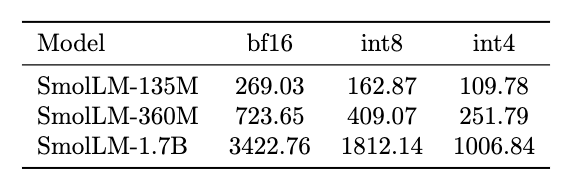
\includegraphics[width=0.8\linewidth]{figures/smollm-memory.png}
}
\end{center}
   \caption{Memory footprint of SmolLM2 models \cite{hf-SmolLM2-usecase}.}
\label{fig:SmolLM2-memory}
\end{figure}


\begin{figure}[t]
\begin{center}
% \fbox{\rule{0pt}{2in} \rule{0.9\linewidth}{0pt}}
\fbox{
    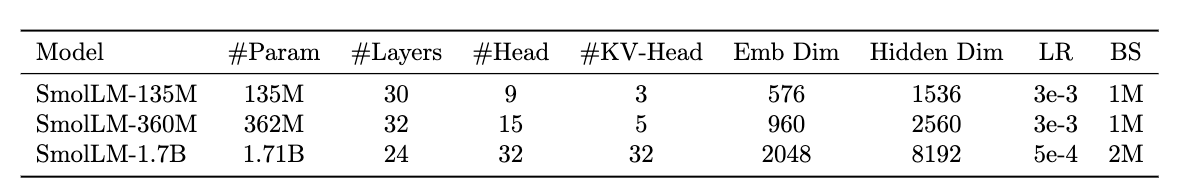
\includegraphics[width=1\linewidth]{figures/smollm-params.png}
}
\end{center}
   \caption{Architecture details of SmolLM2 models \cite{hf-SmolLM2-usecase}.}
\label{fig:SmolLM2-parameteres}
\end{figure}


\subsection{Dataset Selection}
The dataset chosen to test the various models sentiment analysis capabilities was the IMDb's movie Review dataset \cite{IMDB-dataset}. This dataset contains strings of movie reviews, which was pulled from IMDb's website in 2011 making it a sample of the total amount of reviews they store. Each movie review sample is accompanied by the dataset's binary sentiment classification of Positive or Negative. The dataset contains 50,000 total samples with 25,000 being for training and 25,000 for testing with an approximately 50/50 split between Positive and Negative classifications. These specifics of the dataset make it very balanced leading to it being well tested in literature and the perfect benchmark for basic sentiment analysis. Given the datasets format as strings already and it being from the same creators as the models we were testing no pre-processing was needed outside of tokenizing each input prompt before feeding it into the language models. 




%------------------------------------------------------------------------
\section{Approach}

% \textbf{Mention the models were run on A100 with 40gb for consistency among tests}


\subsection{SmolLM2 Choice}
SmolLM2 \cite{hf-SmolLM2-usecase}, developed by Hugging Face, is a family of compact language models designed for efficiency and on-device performance. Available in three sizes—135M, 360M, and 1.7B parameters. Despite their smaller size, SmolLM2 models perform competitively on benchmarks for reasoning, coding, and general knowledge tasks, making them ideal for resource-constrained applications like mobile or edge computing.
We chose SmolLM2 because it is a very recent and efficient model available in extremely small parameter sizes. The fact that it has multiple parameter size is also something we were looking for as it is possible to easily compare the impact of scale by switching between the different parameter size. We focused on the 135M model as the goal of this study is to see the viability of an extremely small LLM for simple NLP tasks. 

% \textbf{Important: Mention any code repositories (with citations) or other sources that you used, and specifically what changes you made to them for your project. }



\subsection{Generating SmolLM2 Benchmarks}
To first investigate or compare the variety of models mentioned some initial tests and benchmarking had to be done. While traditional ML techniques for sentiment analysis and well documented LLMs have existing literature providing metrics for them running on the IMDb dataset \cite{IMDB-dataset} our choice for tuning a SmolLM2 model would require us to determine the baseline performance. Hence one of the first goals of this project was to test all three sizes of SmolLM2 models in both zero-shot and few-shot scenarios so later comparisons could better be made. This benchmarking was done on the 25,000 test samples from the dataset with each sample getting its own individual prompt to the model (no batching was used). The expected outcome of this experiment was that the greater parameter models would perform quite a bit better in terms of accuracy with few-shot learning also outperforming zero-shot in terms of simple accuracy. 

An initial problem which was quickly realized from the zero-shot testing was that the SmolLM2 models did not always return a clear Positive or Negative classification of the movie prompt. Since no previous examples of answering the question were given (few-shot did this) the smaller sized models such as SmolLM2-135M would simple repeat the question back or answer with random commonly used words such as 'I' or The repeatedly. To accommodate for this issue our initial approach had to be adjusted. Rather then parse the full reply that the models generated we took the top 50 most probable next words (logits) that the model generated and parsed through them to see if Positive of Negative appeared and if it did the first one was taken as the models answer. This methodology keeps the premise of sentiment analysis while taking into account that LLMs can give wordy responses making it hard to determine what sentiment they actually gave the prompt. Also, if the model was unable in those 50 most likely words to give an answer of either Positive of Negative this was treated as a default Negative answer however, we tracked these scenarios to bring up in later data points and analysis. 

Another initial testing issue that arose, all of which allowed us to learn about the models better before fine tuning, was the dependence on the prompting method for determining the Models response. For example, if the prompt was phrased as follows: \textit{\textbf{"Only Answer if this Movie Review is Positive or Negative:"}} then the smaller models would be more likely to select the first mentioned classification. So if the prompt asked Positive vs Negative then the model would be biased towards the Positive class. We could not determine a good way to elevate this for the zero-shot testing which is why we set the default class to Negative to assist in biases the choice the other direction. For the more advanced larger models or for the few-shot prompts this was less of an issue but during testing some bias could have been shown to the Positive class. 

Finally, for the few-shot prompting of the models 3 example reviews were used before appending the given sample to the end of them. The 3 example reviews were generated by us and were purposely kept short for the sake of the models interpretation of them, they can be seen in Table \ref{tab:few-shot-prompts}.

\begin{table*}
\begin{center}
% shrinks font as needed to fit the table
\resizebox{\textwidth}{!}{%
\begin{tabular}{|l|l|}
\hline\hline
Few-shot Prompt 1 & 
Movie Review: I loved this movie ! So good plot ! \n Only Answer if this Movie Review is Positive or Negative: Positive \\

Few-shot Prompt 2 & 
Movie Review: I hated this, could be a lot better \n Only Answer if this Movie Review is Positive or Negative: Negative \\

Few-shot Prompt 3 & 
Movie Review: This move was so good I would recommend to all my friends! \n Only Answer if this Movie Review is Positive or Negative: Positive \\
\hline
\end{tabular}
}
\end{center}
\caption{Few-shot prompts used to test default SmolLM2 models.}
\label{tab:few-shot-prompts}
\end{table*}


% \subsection{Gathering Data on LLMs and ML techniques}


\subsection{Fine-tuning SmolLM2-135M}
\label{sec:ft_setup}

In addition to testing out SmolLM2 in zero-shot and few-shot settings, we decided to fine-tune it specifically for the IMDb benchmark. Our approach adapts the pretrained language model for binary sentiment classification (positive/negative), by replacing the original language model's head with a custom classification head. The SmolLM2 weights were frozen, and only the final custom classification head was trained.
This aims to leverage SmolLM2's knowledge about language in general, as the embeddings in the last layer probably have rich context-aware information gained from the successive attention blocks in the Transformer architecture.

It was unclear which token exactly to use the embedding as an input for the final layer. Something that is often done when fine-tuning LLMs is to use the very first token of the sequence's embedding. In that case the sequence would just be the whole paragraph of the movie review. However this did not work well in our experiments.
In the end we chose a prompt resembling a few-shot prompt.

\textit{"example movie review"} ; this movie review is : \textit{positive} ; \textit{"example moview review 2"} ; this movie review is : \textit{negative} ; \textit{"movie review to do inference on"} ; this movie \textbf{review} is :

We then used the embedding from the token highlighted in bold from the last layer of the language model and used this as the input for the custom classification head.


\section{Experiments and Results}
% To calculate the values of accuracy, recall, specificity, precision, and F-score, you need the confusion matrix or the key components: True Positives (TP), True Negatives (TN), False Positives (FP), and False Negatives (FN). Here's how each metric is calculated:

% 1. **Accuracy**: The proportion of correctly classified instances (both positive and negative) out of all instances.
%    \[
%    \text{Accuracy} = \frac{TP + TN}{TP + TN + FP + FN}
%    \]

% 2. **Recall (Sensitivity)**: The proportion of actual positives correctly identified.
%    \[
%    \text{Recall} = \frac{TP}{TP + FN}
%    \]

% 3. **Specificity**: The proportion of actual negatives correctly identified.
%    \[
%    \text{Specificity} = \frac{TN}{TN + FP}
%    \]

% 4. **Precision**: The proportion of predicted positives that are actually positive.
%    \[
%    \text{Precision} = \frac{TP}{TP + FP}
%    \]

% 5. **F-score**: The harmonic mean of precision and recall, balancing the two.
%    \[
%    \text{F-Score} = 2 \cdot \frac{\text{Precision} \cdot \text{Recall}}{\text{Precision} + \text{Recall}}
%    \]


% \textbf{(10 points) How did you measure success? What experiments were used? What were the results, both quantitative and qualitative? Did you succeed? Did you fail? Why? Justify your reasons with arguments supported by evidence and data.}

% \textbf{Important: This section should be rigorous and thorough. Present detailed information about decision you made, why you made them, and any evidence/experimentation to back them up. This is especially true if you leveraged existing architectures, pre-trained models, and code (i.e. do not just show results of fine-tuning a pre-trained model without any analysis, claims/evidence, and conclusions, as that tends to not make a strong project). }



\subsection{Testing Default SmolLM2 Models}
To address the first needed experiment from our approach in the aim of comparing various models some benchmarks had to be created on the 3 types of SmolLM2 models. All three; 135M, 360M, and 1.7B parameter  SmolLM2 models were tested on the test section of the IMDb dataset \cite{IMDB-dataset} with both zero-shot methods and few-shot methods. The results of these experiments are given in Table \ref{tab:default-SmolLM2-metrics} with the models overall accuracy being shown alongside the distribution of classifications which the models made over the prompts. More detailed metrics such as Recall, Specificity, Precision, and F-Score were calculated but are not necessary as relevant to the discussion of comparing these models to the other methods of sentiment analysis due to the dataset being binary and balanced. Instead the sentiment from these advanced metrics is carried over through the discussion of the classifications that the models chose. 

% \begin{table*}
% \begin{center}
% % shrinks font as needed to fit the table
% \resizebox{\textwidth}{!}{%
% \begin{tabular}{|l|c|c|c|c|c|c|c|c|}
% \hline
% Model & Accuracy & Recall & Specificity & Precision & F-Score & \% Positive & \% Negative & \# Unknown \\
% \hline\hline
% SmolLM2-135M Zero-Shot   & 0.50 & 0.01 & 1.00 & 0.78 & 0.02 & 00.78\%  & 99.22\% & 2993  \\

% SmolLM2-360M Zero-Shot   & 0.56 & 1.00 & 0.11 & 0.53 & 0.69 & 94.26\% & 05.74\%  & 2     \\

% SmolLM2-1.7B ~ Zero-Shot & 0.72 & 0.99 & 0.45 & 0.65 & 0.78 & 77.01\% & 22.99\% & 14    \\

% SmolLM2-135M Few-Shot    & 0.59 & 0.80 & 0.37 & 0.56 & 0.66 & 71.86\% & 28.14\% & 0     \\

% SmolLM2-360M Few-Shot    & 0.66 & 0.99 & 0.33 & 0.60 & 0.75 & 82.74\% & 17.26\% & 0     \\

% SmolLM2-1.7B ~ Few-Shot  & 0.81 & 0.99 & 0.62 & 0.73 & 0.84 & 68.48\% & 31.52\% & 0     \\
% \hline
% \end{tabular}
% }
% \end{center}
% \caption{Default SmolLM2 Model's Performance Metrics on IMDb Test Dataset}
% \label{tab:default-SmolLM2-metrics}
% \end{table*}


\begin{table*}[ht]
\centering
\begin{tabular}{|l|c|c|c|c|}
\hline
\textbf{Model} & \textbf{Accuracy} & \textbf{\% Positive} & \textbf{\% Negative} & \textbf{\# Unknown} \\ 
\hline\hline
SmolLM2-135M Zero-Shot   & 0.50 & 00.78\%  & 99.22\% & 2993 \\ 
SmolLM2-360M Zero-Shot   & 0.56 & 94.26\%  & 05.74\% & 2    \\ 
SmolLM2-1.7B ~ Zero-Shot   & 0.72 & 77.01\%  & 22.99\% & 14   \\ 
SmolLM2-135M Few-Shot    & 0.59 & 71.86\%  & 28.14\% & 0    \\ 
SmolLM2-360M Few-Shot    & 0.66 & 82.74\%  & 17.26\% & 0    \\ 
SmolLM2-1.7B ~ Few-Shot    & 0.81 & 68.48\%  & 31.52\% & 0    \\ 
\hline
\end{tabular}
\caption{Default SmolLM2 Model's Performance Metrics on IMDb Test Dataset}
\label{tab:default-SmolLM2-metrics}
\end{table*}

To first analyze the results of the experiment it must be mentioned again that the models had a default sentiment classification of Negative. This is to explain why the percentages of Positive and Negative add up to 100\% yet the models had some choices which were Unknown (the model did not classify). All Unknown predictions were defaulted to Negative for the sake of consistency among the metrics and this did not make a noticeable difference in all of the models besides SmolLM2-135M Zero-Shot. The smallest of the models when using the least advanced method of prompting had many glaring issues, which we sought to fix, but the first of which was its inability to generate a valid classification for \textbf{2,993} samples. When taking into account its lack of classification on the overall accuracy of the model its accuracy goes from \textbf{0.5} to \textbf{0.38} making it by far the worst performing model in this project. 

Furthermore, the SmolLM2-135M Zero-Shot model was the only one to pick majority Negative for the classification at 99.22\% meaning its accuracy of 0.5 or 0.38 was not achieved by any smart methods which would generalize but more so by just picking one of the binary classification options. The reasoning for its preference of the Negative classification over the Positive was an outlier as-well since all other models preferred the positive classification greatly with that preference diminishing as the models went up in parameter size and ability to digest the problem at hand. During testing of the models, as mentioned in the approach, they had a tendency to prefer the classification which was first mentioned to them in the prompt. This effected the zero-shot models more however the SmolLM2-135M model really did just break out of the curve in terms of its predictions or lack their of. 

Overall the experiment was successful as demonstrating a general trend among the models and providing some baseline results for the selected language models. For all of the other models they show the expected trend of few-shot prompting adding about a 10\% increase in performance with the increase in parameters being the largest driving factor in accuracy increases with the best performing model being the SmolLM2-1.7B Few-Shot at 0.81 accuracy. This model also had the most even split between Positive and Negative classifications showing its ability to better understand the prompts being posed. While it still had a bias towards the Positive classification it was able to nearly perfectly predict any Positive prompt correctly while suffering in terms of accuracy due to false positives rather than false negatives. From this benchmarking we took away the importance of few-shot learning for our fine-tuned model and learned many lessons in how the prompts to the language models had to be structured. This also gave a good goal of potential performance to chase as we sought out to beat the best performing default model by using the smallest of the 3 with a Fine-tuned SmolLM23-135M. 


\subsection{Comparison Between LLMs, Traditional ML, and SmolLM2s}
The goal of this experiment is to compare the performance and costs of various sentiment analysis techniques, demonstrating that there are efficient and comparable alternatives to LLMs for sentiment analysis tasks. LLMs, while impressive and effective at sentiment analysis tasks, are computationally demanding and are not suitable for environments that cannot afford to support high performance computing. This experiment compares LLMs with naive bayes, random forests, logistic regression, and SLMs, to provide a comprehensive discussion on the alternative resources for sentiment analysis tasks to LLMs. The models are compared by measuring their accuracy, precision, recall, training time, and model size. The naive bayes, random forest, and logistic regression models all use TF-IDF to improve their performance outcome by reducing the influence of common terms, terms like “the”, “and”, etc. Understanding the alternatives to LLMs for sentiment analysis tasks enables the development of efficient, resource conscious solutions for sentiment analysis tasks for users and businesses who may not have the resources to use LLMs.

The naive bayes model was determined to be a satisfactory alternative to LLMs for simple sentiment analysis tasks, and for users who are okay with lower accuracy in exchange for significantly reduced memory usage and training time. Naive bayes models store conditional probabilities for each feature/class, resulting in their memory size increasing linearly with the number of features/classes. Compared to LLMs, whose size depends on their millions or billions of parameters, naive bayes models are significantly smaller. In addition, naive bayes models are simple to train, training in just O(n*d), where n is the number of samples, and d is the number of features. This is due to the relatively simple calculations needed to compute the conditional probabilities of words and classes for each sentiment sample. Its performance on complex textual samples is hindered by its interpretation of each word as independent, resulting in erroneous classifications on samples that have conflicting word/sentiment probabilities. For example, a review that says “This movie was so good it made me want to ignore the whole thing and scroll on my phone instead” might be incorrectly classified as a positive review due to the high weight that “good” places on the positive review class probability. However, for simple texts such as those in the IMDb dataset, naive bayes achieved decent results: 0.8228 accuracy, 0.8285 precision, and 0.8174  recall \cite{MLTechniques}. These results indicate that the naive bayes model can correctly assign the correct sentiment class most of the time, but still has significant error. 

The random forest model was determined to be a dissatisfactory alternative to LLMs due to its relatively high memory usage and training times, and no significant improvement in results. Random forests can be large due to their size multiplicatively increasing with the number of trees, nodes, and features. In addition, random forests are trained in a time of O(t*s*f*d), where t is the number of trees, s is the number of samples, f is the number of features, and d is the average tree depth. Training time can be significantly increased with the size of the forest/dataset, and is lengthy when compared to naive bayes models, or other, similarly less complex models. When run on the IMDb dataset, the random forest model did not achieve significantly higher results than the naive bayes: 0.8562 accuracy, 0.8597 precision, 0.8539 recall \cite{MLTechniques}. While smaller and faster to train than LLMs, random forests are not satisfactory alternatives due to still demanding relatively high memory and time resources, without the significant increase in results.

Logistic regression was determined to be a good alternative to LLMs due to its high results on the IMDb dataset, and its satisfactory size and training times when compared to random forests. Logistic regression’s memory needs are dependent solely on the number of features, where random forests must account for many trees, which may have many branching subtrees/nodes. In addition, the  logistic regression model trains in a time of O(d*k), where d is the number of features, and k is the number of iterations. While slower to train than naive bayes, the significantly higher results make it a comparable choice. When run on the IMDb dataset, the logistic regression model achieved high results: 0.8914 accuracy, 0.882 precision, and 0.9055 recall \cite{MLTechniques}. These results are comparable to LLMs, especially when the significantly lower memory requirements and training times of the logistic regression model is considered. For users who demand high results, and have decent resources for memory and training time, the logistic regression model is a good alternative to LLMs.

SmolLM2-135M was determined to be a good alternative to LLMs for sentiment analysis tasks due to its high accuracy. However, it is a less ideal alternative compared to logistic regression due to its slower training time and larger model size. SmolLM2-135M achieved 0.892 accuracy on the IMDb dataset performing sentiment analysis. This is comparable to both logistic regression and LLMs. SmolLM2-135M is faster to train than LLMs due to having only 135 million parameters compared to ChatGPT’s 1.7 billion. In addition, having significantly less parameters means that SmolLM2-135M is much smaller in size and requires less memory resources for use on sentiment analysis tasks. Being able to achieve high accuracy results within 2 percentage points of LLMs, and being much smaller and faster to train, make SmolLM2-135M a good alternative to LLMs for sentiment analysis applications. However, SmolLM2-135M is a neural network based model, and results in a computationally intensive training process when compared to logistic regression. This, in addition to logistic regression’s comparatively small size, make it a more suitable choice for a LLM alternative in most sentiment analysis use cases. 

This experiment was successful in identifying alternative models to LLMs for sentiment analysis applications. Logistics regression with TF-IDF was determined to be the ideal alternative, due to its high accuracy results, relatively fast training times, and compact model size. Logistic regression performed very well in terms of accuracy, reaching within 2 percentage points of LLMs. In most scenarios, logistic regression will provide comparable performance at a much lower cost. Naive bayes was the fastest model to train and smallest in size, but fell 10 percentage points from LLMs in terms of classification accuracy. In use cases where speed and space are a tighter constraint than accuracy, naive bayes is a good alternative to LLMs. SmolLM2-135M delivered accuracy results equivalent to logistic regression but was much slower to train and significantly larger in size, making it a less favorable alternative to LLMs when compared to logistic regression. Random forests proved to be a poor alternative due to their high training times and larger size relative to other alternatives, without achieving competitive accuracy. While these lightweight models are effective for general sentiment analysis tasks, there are scenarios where LLMs offer distinct advantages. For instance, LLMs excel in understanding nuanced language features such as sarcasm, irony, or context-dependent sentiment shifts, which simpler models may struggle to capture. In conclusion, we can confidently say that lightweight, high-performing models are viable alternatives for sentiment analysis applications, offering efficient solutions without the resource demands of LLMs. Among these, logistic regression with TF-IDF stands out as the most efficient option, balancing accuracy, speed, and compactness.



\begin{table*}
\begin{center}
% shrinks font as needed to fit the table
\resizebox{\textwidth}{!}{%
\begin{tabular}{|l|c|c|c|c|c|c|c|c|}
\hline
Model with TF-IDF & Accuracy & Precision & Recall & F-Score & AUC \\
\hline\hline
Naive Bayes   & 0.8228 & 0.8285 & 0.8174 & 0.823 & 0.85   \\

Random Forest   & 0.8562 & 0.8597 & 0.8539 & 0.8568 & 0.93  \\

Logistic Regression  & 0.8914 & 0.882 & 0.9055 & 0.8936 & 0.96     \\


\hline
\end{tabular}
}
\end{center}
\caption{ML techniques Performance on IMDb Dataset}
\label{tab:large-models-metrics}
\end{table*}


\begin{table*}
\begin{center}
% shrinks font as needed to fit the table
\resizebox{\textwidth}{!}{%
\begin{tabular}{|l|c|c|c|c|c|c|c|c|}
\hline
Model & Accuracy & Recall & Specificity & Precision & F-Score & \% Positive & \% Negative & \# Unknown \\
\hline\hline
SmolLM2-135M Zero-Shot   & 0.50 & 0.01 & 1.00 & 0.78 & 0.02 & 00.78\%  & 99.22\% & 2993  \\

SmolLM2-360M Zero-Shot   & 0.56 & 1.00 & 0.11 & 0.53 & 0.69 & 94.26\% & 05.74\%  & 2     \\

SmolLM2-1.7B ~ Zero-Shot & 0.72 & 0.99 & 0.45 & 0.65 & 0.78 & 77.01\% & 22.99\% & 14    \\

SmolLM2-135M Few-Shot    & 0.59 & 0.80 & 0.37 & 0.56 & 0.66 & 71.86\% & 28.14\% & 0     \\

SmolLM2-360M Few-Shot    & 0.66 & 0.99 & 0.33 & 0.60 & 0.75 & 82.74\% & 17.26\% & 0     \\

SmolLM2-1.7B ~ Few-Shot  & 0.81 & 0.99 & 0.62 & 0.73 & 0.84 & 68.48\% & 31.52\% & 0     \\
\hline
\end{tabular}
}
\end{center}
\caption{Large Models' Performance on IMDb Dataset}
\label{tab:large-models-metrics}
\end{table*}




\subsection{Results of Fine-tuning SmolLM2-135M}

We used the experimental setup described in section \ref{sec:ft_setup}.
We trained for a total of 10 epochs using the whole trainig dataset, with 
\begin{figure}
    \centering
    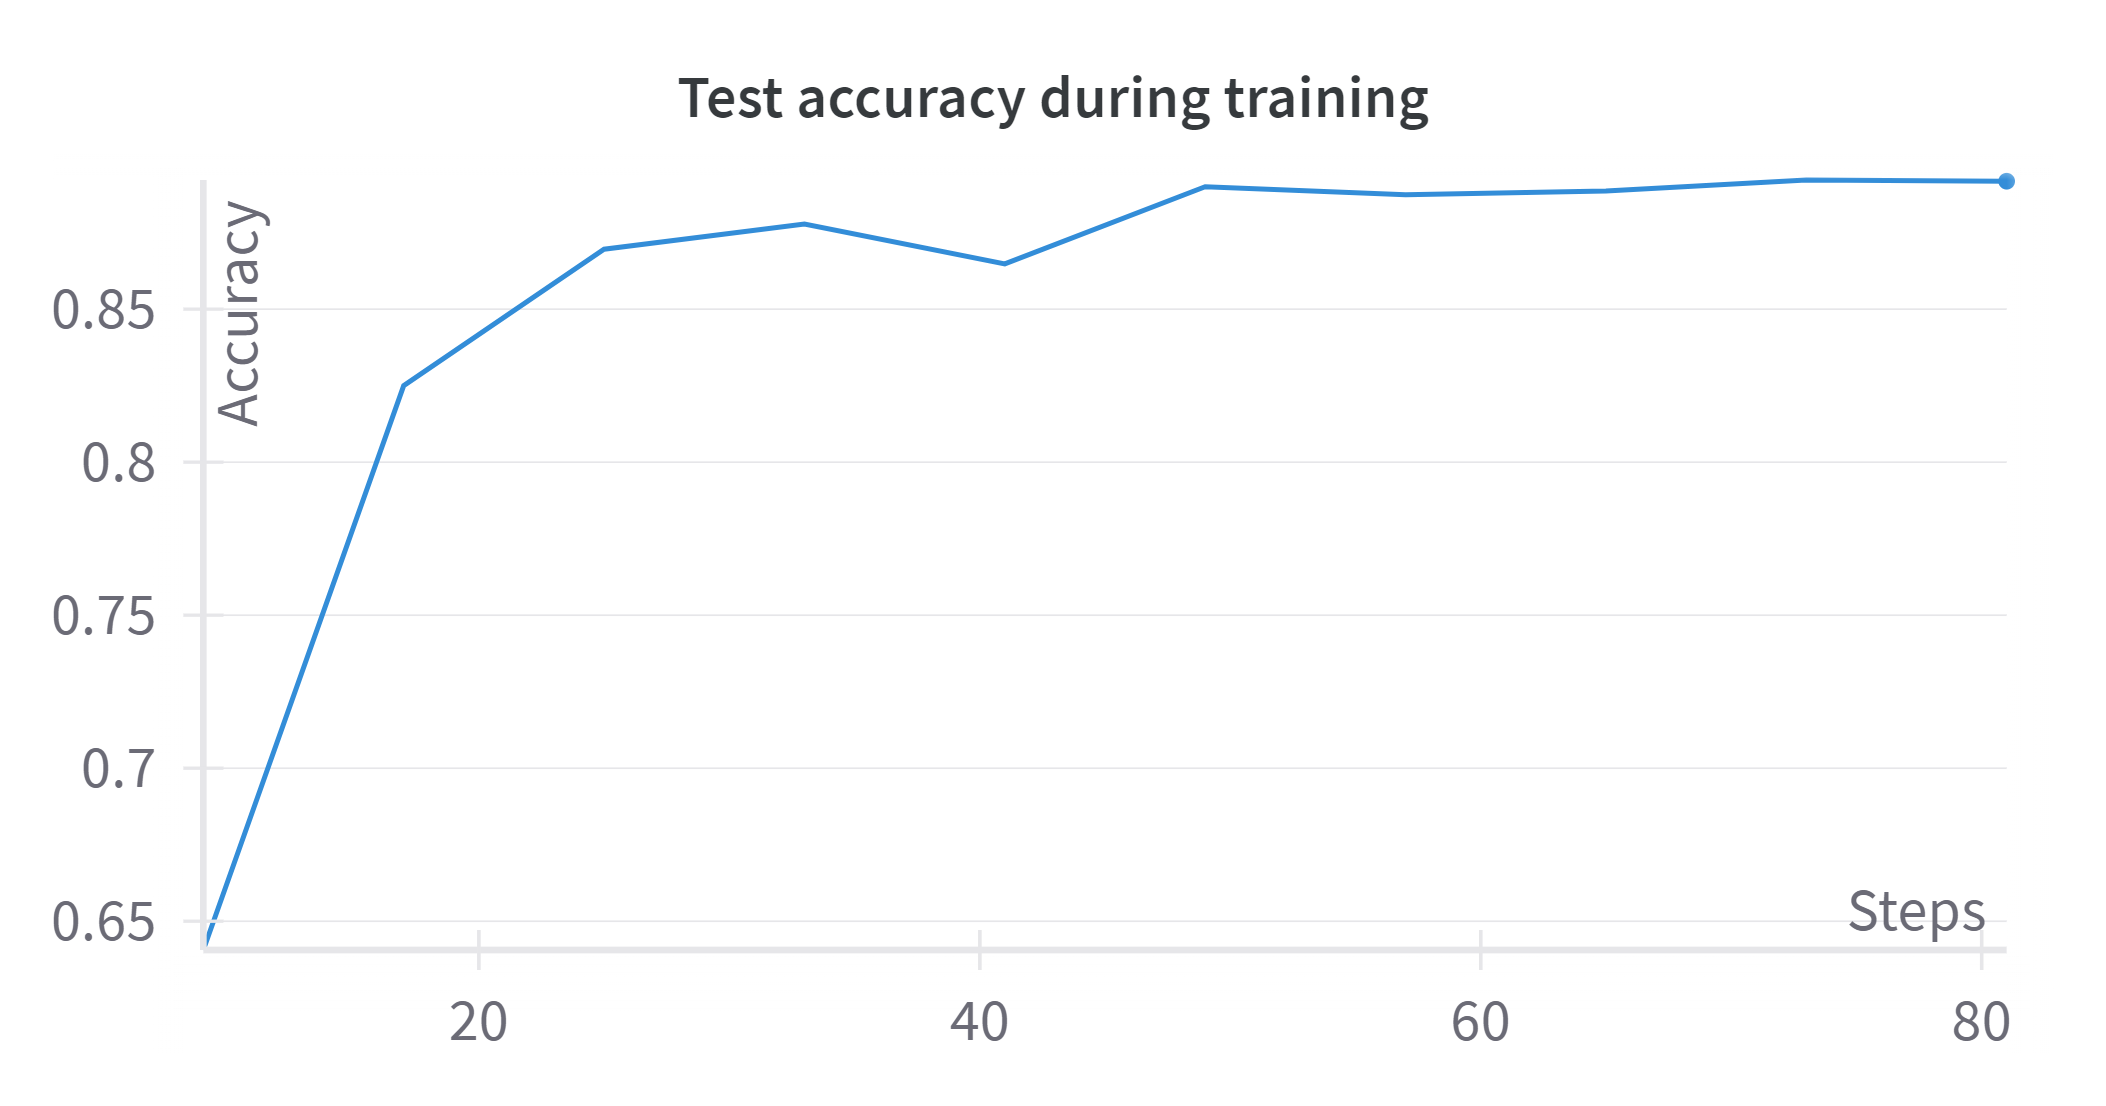
\includegraphics[width=1\linewidth]{figures/W&B Chart 12_10_2024, 1_55_29 PM.png}
    \caption{Fine-tuning SmolLM2 for 10 epochs with final accuracy reaching 89.2\%}
    \label{fig:enter-label}
\end{figure}
\textbf{recompare and give data and why stuff was how it was}


lr : 1e-4 with 120 warmup steps
4 GPUS batch size 90 per device
10 epochs
0.01 weight decay
0.2 warmup
576 -> 384 -> 2 with cross entropy loss, batchnorm, gelu activation
dropout

Ours gets almost 90\%, tried out different architectures etc, most get 88\%, best gets 89.1\% or more.
probably possible to squeeze out 90\% from SmolLM2, and more with bigger param size / ensembling with different prompt setups.

GPT 2 finetuned gets     92.36 accuracy

%-------------------------------------------------------------------------
\section{Conclusion}
In this project, we evaluated several smaller language models and ultimately selected the SmolLM2 model for fine-tuning. SmolLM2 stands out as a recent and highly efficient option, available in a range of parameter sizes, the sizes that we focused on were the 135M, 360M, and 1.7B models. 

First we tested and evaluated these models using both zero-shot and few-shot approaches and we successfully demonstrated an expected general trend that few shot prompting adds about a 10\% increase in performance. Our analysis also revealed that increasing parameter size was the most significant factor in improving accuracy. 
We also researched various different traditional machine learning methods for sentiment analysis, such as Naive Bayes, Random Forest classifiers, and Logistic Regression models. Our analysis of the different machine learning methods demonstrated that traditional machine learning methods have a strong performance without the expensive resources of LLMs. The most competitive traditional machine learning model was the Logistic Regression with TF-IDF with an accuracy of 89.14\%.

We also experimented with the SmolLM2-135M’s hyperparameters to see if we were able to fine tune the model well enough to be competitive to larger models. Our fine tuned SmolLM2-135M was able to achieve an accuracy of 89.2\%, which is fairly competitive to GPT 2’s accuracy of 92.36\%. This experiment highlights the importance of fine tuning, particularly for smaller models, and it also highlights their potential to deliver high quality results with significantly less resources.
Upon completing these experiments,  we found that we were able to fine-tune the SmolLM2 well enough to achieve accuracy results comparable to GPT-2. We also concluded that traditional machine learning models, specifically the Logistic Regression model with TF-IDF gives us the most competitive performance with fairly low costs and accuracy results that are comparable to the SmolLM2. Despite being computationally expensive, larger models are still valuable in sentiment analysis for particular scenarios that require very high accuracy and/or also have very particular nuances, like wanting the model to understand irony, sarcasm, etc. 








% You are welcome to introduce additional sections or subsections, if required, to address the following questions in detail. 

% (5 points) Appropriate use of figures / tables / visualizations. Are the ideas presented with appropriate illustration? Are the results presented clearly; are the important differences illustrated? 

% (5 points) Overall clarity. Is the manuscript self-contained? Can a peer who has also taken Deep Learning understand all of the points addressed above? Is sufficient detail provided? 

% (5 points) Finally, points will be distributed based on your understanding of how your project relates to Deep Learning. Here are some questions to think about: 

% What was the structure of your problem? How did the structure of your model reflect the structure of your problem? 

% What parts of your model had learned parameters (e.g., convolution layers) and what parts did not (e.g., post-processing classifier probabilities into decisions)? 

% What representations of input and output did the neural network expect? How was the data pre/post-processed?
% What was the loss function? 

% Did the model overfit? How well did the approach generalize? 

% What hyperparameters did the model have? How were they chosen? How did they affect performance? What optimizer was used? 

% What Deep Learning framework did you use? 

% What existing code or models did you start with and what did those starting points provide? 

% Briefly discuss potential future work that the research community could focus on to make improvements in the direction of your project's topic.


%-------------------------------------------------------------------------

\section{Work Division}

A summary of each authors contributions are provided in Table \ref{tab:contributions}.



% \section{Miscellaneous Information}

% The rest of the information in this format template has been adapted from CVPR 2020 and provides guidelines on the lower-level specifications regarding the paper's format.

% \subsection{Language}

% All manuscripts must be in English.


% \subsection{Paper length}
% Papers, excluding the references section,
% must be no longer than six pages in length. The references section
% will not be included in the page count, and there is no limit on the
% length of the references section. For example, a paper of six pages
% with two pages of references would have a total length of 8 pages.

% %-------------------------------------------------------------------------
% \subsection{The ruler}
% The \LaTeX\ style defines a printed ruler which should be present in the
% version submitted for review.  The ruler is provided in order that
% reviewers may comment on particular lines in the paper without
% circumlocution.  If you are preparing a document using a non-\LaTeX\
% document preparation system, please arrange for an equivalent ruler to
% appear on the final output pages.  The presence or absence of the ruler
% should not change the appearance of any other content on the page.  The
% camera ready copy should not contain a ruler. (\LaTeX\ users may uncomment
% the \verb'\cvprfinalcopy' command in the document preamble.)  Reviewers:
% note that the ruler measurements do not align well with lines in the paper
% --- this turns out to be very difficult to do well when the paper contains
% many figures and equations, and, when done, looks ugly.  Just use fractional
% references (e.g.\ this line is $095.5$), although in most cases one would
% expect that the approximate location will be adequate.

% \noindent
% FAQ\medskip\\
% {\bf Q:} Are acknowledgements OK?\\
% {\bf A:} No.  Leave them for the final copy.\medskip\\
% {\bf Q:} How do I cite my results reported in open challenges?
% {\bf A:} To conform with the double blind review policy, you can report results of other challenge participants together with your results in your paper. For your results, however, you should not identify yourself and should not mention your participation in the challenge. Instead present your results referring to the method proposed in your paper and draw conclusions based on the experimental comparison to other results.\medskip\\

% \begin{figure}[t]
% \begin{center}
% \fbox{\rule{0pt}{2in} \rule{0.9\linewidth}{0pt}}
%    %\includegraphics[width=0.8\linewidth]{egfigure.eps}
% \end{center}
%    \caption{Example of caption.  It is set in Roman so that mathematics
%    (always set in Roman: $B \sin A = A \sin B$) may be included without an
%    ugly clash.}
% \label{fig:long}
% \label{fig:onecol}
% \end{figure}

% \begin{figure*}
% \begin{center}
% \fbox{\rule{0pt}{2in} \rule{.9\linewidth}{0pt}}
% \end{center}
%    \caption{Example of a short caption, which should be centered.}
% \label{fig:short}
% \end{figure*}

% %------------------------------------------------------------------------
% \subsection{Formatting your paper}

% All text must be in a two-column format. The total allowable width of the
% text area is $6\frac78$ inches (17.5 cm) wide by $8\frac78$ inches (22.54
% cm) high. Columns are to be $3\frac14$ inches (8.25 cm) wide, with a
% $\frac{5}{16}$ inch (0.8 cm) space between them. The main title (on the
% first page) should begin 1.0 inch (2.54 cm) from the top edge of the
% page. The second and following pages should begin 1.0 inch (2.54 cm) from
% the top edge. On all pages, the bottom margin should be 1-1/8 inches (2.86
% cm) from the bottom edge of the page for $8.5 \times 11$-inch paper; for A4
% paper, approximately 1-5/8 inches (4.13 cm) from the bottom edge of the
% page.

% %-------------------------------------------------------------------------
% \subsection{Margins and page numbering}

% All printed material, including text, illustrations, and charts, must be kept
% within a print area 6-7/8 inches (17.5 cm) wide by 8-7/8 inches (22.54 cm)
% high.



% %-------------------------------------------------------------------------
------------------------------------------------------------


\newpage

{\small
\bibliographystyle{ieee_fullname}
\bibliography{dl-fp-refrences}
}


\newpage

\section{A. Project Code Repository}
The Github repository containing the experiments mentioned throughout the report alongside the default and tuned models can be found \hyperlink{https://github.com/jadenzwicker/DL-Final-Project/tree/main}{here}. 






% Table of participation
\newpage

\begin{table*}
\begin{center}
% shrinks font as needed to fit the table
\resizebox{\textwidth}{!}{%
\begin{tabular}{|l|c|p{8cm}|}
\hline
Student Name & Contributed Aspects & Details \\
\hline\hline
Jaden Zwicker & Default Model Experimentation \& Analysis & 
Performed various experiments on the 3 SmolLM2 models in their default configuration. Analyzed the results of these experiments to compare and contrast them with the larger LLMs and to set a baseline of performance before fine tuning. 
\\

Houshmand Abbaszadeh & Analysis \& Comparison of Various ML Techniques & Performed an experiment to compare different ML techniques for sentiment analysis applications, successfully identifying alternative models to LLMs for sentiment analysis. Analyzed and documented the results of the experiment, as well as contributing to the abstract, introduction, and approach sections of the paper.  \\

Brieuc Popper & SmolLM2 finetuning, general coding tasks & Designed and ran the fine-tuning experiments with SmolLM2-135M. Helped team setup on PACE ICE GPUs and all around Python Code with \textit{transformers} library to deal with LLMs \\

\hline
\end{tabular}
}
\end{center}
\caption{Contributions of team members.}
\label{tab:contributions}
\end{table*}





\end{document}
